% -----------------------------------------------------------------------------
%
% Copyright (c) 2017 Sam Cox, Roberto Sommariva
%
% This file is part of the AtChem2 software package.
%
% This file is covered by the MIT license which can be found in the file
% LICENSE.md at the top level of the AtChem2 distribution.
%
% -----------------------------------------------------------------------------

\chapter{Model Setup} \label{ch:setup}

% -------------------------------------------------------------------- %
\section{Chemical Mechanism} \label{sec:chemical-mechanism}

The chemical mechanism is the core element of an atmospheric chemistry
model. In AtChem2, the mechanism file is written in FACSIMILE format
and has the extension \texttt{.fac}. The FACSIMILE format is used to
describe chemical reactions in the commercial
\href{http://www.mcpa-software.com/}{FACSIMILE Kinetic Modelling Software};
for historical reasons, the software and the format have been
often used in conjunction with the MCM. The
\href{http://mcm.leeds.ac.uk/MCM/extract.htt}{extraction tool} on the
MCM website can generate \texttt{.fac} files directly in FACSIMILE
format (see Sect.~\ref{subsec:mcm-extraction}).

\subsection{The FACSIMILE format} \label{subsec:facsimile-format}

Chemical reactions are described in FACSIMILE format using the
following notation:

\begin{verbatim}
% k : A + B = C + D ;
\end{verbatim}

where \texttt{k} is the rate coefficient, \texttt{A} and \texttt{B}
are the reactants, \texttt{C} and \texttt{D} are the products. A
reaction starts with the \texttt{\%} character and ends with the
\texttt{;} character. Comments can be inserted in the \texttt{.fac}
file to document and annotate the chemical mechanism: in FACSIMILE
format, comments are enclosed between the characters \texttt{*} and
\texttt{;} and are ignored by the build scripts.

The rate coefficient (\texttt{k}) can be a constant number or, more
commonly, can be calculated as a function of other variables, such as
temperature (\texttt{TEMP}), air density (\texttt{M}), water vapour
(\texttt{H2O}) and other environment variables
(Sect.~\ref{sec:environment-variables}). A basic chemical mechanism,
with comments and calculated rate coefficients, looks like this:

\begin{verbatim}
* Tropospheric O3-NOx cycle ;
* Kinetic data from Atkinson et al., ACP, 2004 ;
% J_NO2                      : NO2 = NO + O ;
% 5.6D-34*M*(TEMP/300)@-2.6  : O + O2 = O3 ;
% 1.4D-12*EXP(-1310/TEMP)    : NO + O3 = NO2 + O2 ;
\end{verbatim}

The photolysis rate of \cf{NO2} (\texttt{J\_NO2}) in the example above
is calculated by AtChem2 as function of latitude, longitude and solar
zenith angle, as explained in detail in Sect.~\ref{sec:photolysis-rates}.
Complex mathematical expressions can be used to calculate the rate
coefficient, in which case they have to be defined before the chemical
reactions that use them (typically, combination and dissociation
reactions). For example:

\begin{verbatim}
* Formation of nitric acid (HNO3) in the gas-phase ;
*;
* Rate coefficient (Atkinson et al., ACP, 2004) ;
K80 = 3.3D-30*M*(TEMP/300)@-3.0 ;
K8I = 4.1D-11 ;
KR8 = K80/K8I ;
FC8 = 0.4 ;
NC8 = 0.75-1.27*(LOG10(FC8)) ;
F8 = 10@(LOG10(FC8)/(1+(LOG10(KR8)/NC8)**2)) ;
KMT08 = (K80*K8I)*F8/(K80+K8I) ;
*;
* Chemical Reaction ;
% KMT08 : OH + NO2 = HNO3 ;
\end{verbatim}

Chemical reactions can be written in FACSIMILE format without
reactants or products. This feature is useful to implement simple
descriptions of non-chemical processes in a box-model. For example,
dry deposition to the surface and direct emission of a chemical
species can be parametrized as:

\begin{verbatim}
* Deposition velocity of O3 = 1.4 cm s-1 ;
% 1.4/BLHEIGHT  :  O3 =  ;

* Emission rate of NO2 = 1e8 molecule cm-3 s-1 ;
% 1D+8  :  = NO2  ;
\end{verbatim}

More sophisticated approaches to describe non-chemical processes can
be implemented either by defining complex mathematical expressions to
calculate the corresponding ``rate coefficients'' (as shown above) or
by writing the appropriate Fortran function(s) into the source code.

The \texttt{.fac} file is processed by a Python script
(\texttt{mech\_converter.py}, see Sect.~\ref{subsec:build-process});
the script expects the chemical mechanism to have four sections:

\begin{description}
\item[Generic rate coefficients] : contains the definitions of the
  generic rate coefficients used when experimental kinetic data are
  not available.
\item[Complex reactions] : contains the mathematical expressions to
  calculate complex rate coefficients (e.g., for combination and
  dissociation reactions).
\item[Peroxy radicals] : contains the calculation of the \cf{RO2} sum
  -- go to Sect.~\ref{subsec:ro2-sum} for details.
\item[Reaction definitions] : contains the chemical reactions (and
  parametrized non-chemical processes) in FACSIMILE format.
\end{description}

For \texttt{mech\_converter.py} to work, the beginning of each section
must be delimited by a header constituted by a single comment line.
The header must always be present, even though the corresponding
sections can be empty. A minimal \texttt{.fac} file
(\texttt{mechanism\_skel.fac}) and an example chemical mechanism
downloaded from the MCM website (\texttt{mechanism\_test.fac}) are
included in the \texttt{mcm/} directory for reference and testing.

\subsection{The \cf{RO2} sum} \label{subsec:ro2-sum}

The sum of organic peroxy radicals (\cf{RO2}) is a key feature of the
Master Chemical Mechanism. Organic peroxy radicals react with
\cf{HO2}, with themselves and with other \cf{RO2}: given that there
are over 1000 peroxy radicals in the MCM, the number of possible self
and cross reactions is of the order of $10^6$, which presents a
significant computational challenge. The \cf{RO2} sum is used in the
MCM to keep the number of peroxy radicals permutation reactions to a
reasonable number, as explained in the MCM protocol papers
\citep{jenkin_1997, saunders_2003}.

AtChem2 is designed primarily to run models based upon the MCM, and
therefore the \texttt{.fac} file must contain a section with the
calculation of the \cf{RO2} sum (Sect.~\ref{subsec:facsimile-format}).
This section must have a header and has the following format:

\begin{verbatim}
* Peroxy radicals. ;
RO2 = RO2a + RO2b + RO2c + ... ;
\end{verbatim}

where \texttt{RO2a}, \texttt{RO2b}, \texttt{RO2c}, are the organic
peroxy radicals in the chemical mechanism. If there are no organic
peroxy radicals in the chemical mechanism (or if the mechanism is not
based upon the MCM), the \cf{RO2} sum section must still be present in
the \texttt{.fac} file, but it is left empty:

\begin{verbatim}
* Peroxy radicals. ;
RO2 = ;
\end{verbatim}

The \cf{RO2} sum is automatically generated from the chemical
mechanism during the build process using the list of \cf{RO2}
extracted from the MCM database (Sect.~\ref{subsec:build-process}).
AtChem2 includes the complete list of all organic peroxy radicals in
the MCM v3.3.1 (\texttt{mcm/peroxy-radicals\_v3.3.1}), which is the
version used by default. Complete lists of all organic peroxy radicals
in the other versions of the MCM are also included in the
\texttt{mcm/} directory. Instructions on how to set up AtChem2 to use
the previous versions of the MCM can be found in the file
\texttt{mcm/INFO.md}. The value of the \cf{RO2} sum is always output
together with the environment variables (in
\texttt{model/output/environmentVariables.output}).

It is important to ensure that the \cf{RO2} sum is accurate, because
many reactions in the MCM use the value of this parameter to calculate
the reaction rate correctly. The hydroperoxyl radical (\cf{HO2}) is a
peroxy radical but is not an organic molecule, and therefore it
\emph{should not} be included in the \cf{RO2} sum.

\subsection{MCM extraction} \label{subsec:mcm-extraction}

The MCM website provides a convenient tool that can be used to
download the whole Master Chemical Mechanism (or subsets of it) in
FACSIMILE format. Only a brief overview of the process will be given
here: for more information go to the \href{http://mcm.leeds.ac.uk/}{MCM website}.

First, select the species of interest using the
\href{http://mcm.leeds.ac.uk/MCM/roots.htt}{MCM browser} and add the
selection to the \emph{Mark List}. Then proceed to the
\href{http://mcm.leeds.ac.uk/MCM/extract.htt}{MCM extraction tool} and
select the option \emph{FACSIMILE input format, suitable for inserting
  into a FACSIMILE model.}. Make sure that the following options are
selected, so that the required headers (Sect.~\ref{subsec:facsimile-format})
will be included in the generated \texttt{.fac} file: :

\begin{verbatim}
[x] Include inorganic reactions?
[x] Include generic rate coefficients?
    FACSIMILE, FORTRAN and KPP formats only
\end{verbatim}

Click on \emph{Extract} to download the \texttt{.fac} file into a
directory of choice -- such as the \texttt{model/} directory, as
discussed in Sect.~\ref{sec:model-structure}. The downloaded
\texttt{.fac} file is a simple text file and can be used directly in
AtChem2. If modifications are required (e.g., if you want to add,
delete, or change some chemical reactions) open the \texttt{.fac} file
with a text editor and edit the chemical mechanism as needed.

\subsection{The build process} \label{subsec:build-process}

AtChem2 is built using the set of scripts in the \texttt{build/}
directory. Here, we only outline the build process; detailed
instructions on how to build the model can be found in
Sect.~\ref{sec:build}.

The Python script \texttt{mech\_converter.py}, which is automatically
called by the \texttt{build\_atchem2.sh} script, converts the chemical
mechanism from the FACSIMILE fortmat into a format that can be read by
the Fortran code. In doing so, the Python script generates a number of
files:

\begin{itemize}
\item \texttt{mechanism.f90} contains the equations, in Fortran code,
  to calculate the rate coefficients of each reaction of the chemical
  mechanism.
\item \texttt{mechanism.so} is the shared library, i.e. the
  pre-compiled version of the chemical mechanism.
\item \texttt{mechanism.species} contains the list of chemical species
  in the chemical mechanism. The file has no header. The first column
  is the \emph{ID number} of the species, the second column is the
  name of the species:
  \begin{verbatim}
  1 O
  2 O3
  3 NO
  4 NO2
  \end{verbatim}
\item \texttt{mechanism.reac} and \texttt{mechanism.prod} contain the
  reactants and the products (respectively) in each reaction of the
  chemical mechanism. The files have a one line header with the number
  of species, the number of reactions and the number of equations in
  the \emph{Generic rate coefficients} and \emph{Complex reactions}
  sections (Sect.~\ref{subsec:facsimile-format}). The first column is
  the \emph{ID number} of the reaction, the second column is the
  \emph{ID number} of the chemical species which are
  reactants/products in that reaction:
  \begin{verbatim}
  29 71 139 numberOfSpecies numberOfReactions numberOfGenericComplex
  1 1
  2 1
  3 1
  3 2
\end{verbatim}
\item \texttt{mechanism.ro2} contains the organic peroxy radicals
  (\cf{RO2}). The file has a one line header formatted as a Fortran
  comment. The first column is the \emph{ID number} of the peroxy
  radical (from \texttt{mechanism.species}), the second column is the
  name of the peroxy radical as a Fortran comment:
  \begin{verbatim}
  ! Note that this file is generated by build/mech_converter.py
  ! based upon the file mcm/mechanism_test.fac
  ! Any manual edits to this file will be overwritten when
  ! calling build/mech_converter.py
  23 !CH3O2
  26 !C2H5O2
  28 !IC3H7O2
  29 !NC3H7O2
  \end{verbatim}
\end{itemize}

The directory containing the files generated by the build script is
the \sharedir\ which, by default, is \texttt{model/configuration/}:
the location of the \sharedir\ can be changed using the second
argument of the build script, as explained in more detail in
Sect.~\ref{sec:build} (see also Sect.~\ref{subsec:model-directory}).

% -------------------------------------------------------------------- %
\section{Model Parameters} \label{sec:model-parameters}

The model parameters control the general setup of the model; they are
set in the \texttt{model.parameters} file which, by default, is
in the \texttt{model/configuration/} directory.

\begin{itemize}
\item \textbf{number of steps} and \textbf{step size}. The duration of
  the model run is determined by the number of steps and by the step
  size (in seconds). The step size controls the frequency of the model
  output for the chemical species listed in \texttt{outputSpecies.config}
  (Sect.~\ref{sec:config-files}), as well as for all the environment
  variables, the photolysis rates and the diagnostic variables. The
  step size is not related to the integration step
  which is controlled by CVODE.\\
  For example, a model runtime of 2 hours, with output every 5
  minutes, requires 24 steps with a step size of 300 seconds (24x300 =
  7200 sec = 2 hours).
\item \textbf{species interpolation method} and
  \textbf{conditions interpolation method}. Interpolation method used
  for the constrained chemical species, and for the constrained
  environment variables and the photolysis rates, respectively
  (Sect.~\ref{sec:constraints}). Two interpolation methods are
  currently implemented in AtChem2: piecewise constant and piecewise
  linear. The default option is \texttt{2} (piecewise linear
  interpolation).
\item \textbf{rates output step size}. Frequency (in seconds) of the
  model output for the production and loss rates of selected chemical
  species, i.e. those listed in \texttt{outputRates.config}
  (Sect.~\ref{sec:config-files}).
\item \textbf{model start time}. Start time of the model (in seconds)
  calculated from midnight of the \textbf{day}, \textbf{month},
  \textbf{year} parameters (see below). For example, a start time of
  3600 means the model run starts at 1:00 in the morning and a start
  time of 46800 means the model run starts at 1:00 in the afternoon
  (13:00). The \textbf{model stop time} is automatically calculated by
  the model as:
  \begin{verbatim}
  model start time + (number of steps * step size)
  \end{verbatim}
  \emph{N.B.:} when one or more variables are constrained, the time
  interval between the model start time and the model stop time
  \emph{must be} equal to or less than the time interval of the
  constrained data (Sect.~\ref{sec:constraints}).
\item \textbf{jacobian output step size}. Frequency (in seconds) of
  the model output for the Jacobian matrix. If this parameter is set
  to \texttt{0} (default option), the Jacobian matrix is not
  output. Note that the \texttt{jacobian.output} file generated by the
  model can be very large, especially if the chemical mechanism has
  many reactions and/or the model runtime is long.
\item \textbf{latitude} and \textbf{longitude}. Geographical
  coordinates (in degrees). Latitude North is positive and latitude
  South is negative; longitude East is negative and longitude West is
  positive~\footnote{The preferred convention is that longitude East
    is positive and longitude West is negative. The current version of
    AtChem2 uses the opposite convention to maintain compatibility
    with previous versions.}. Latitude and longitude are used to
  calculate the Earth-Sun angles, which are needed for the calculation
  of the photolysis rates (Sect.~\ref{sec:photolysis-rates}).
\item \textbf{day} and \textbf{month} and \textbf{year}. Start date of
  the model simulation. The model time is in UTC (GMT timezone) and is
  calculated in seconds since midnight of the start date.
\item \textbf{reaction rates output step size}. Frequency (in seconds)
  of the model output for the reaction rates of every reaction in the
  chemical mechanism. By default, the reaction rates are saved in the
  directory \texttt{model/output/reactionRates/} as one file for each
  model step, with the name of the file corresponding to the time in
  seconds. In previous versions of AtChem, this output was called
  \textbf{instantaneous rates}. This parameter is different from
  \textbf{rates output step size} (see above), which sets the
  frequency of a formatted output of reaction rates for selected
  species of interest. For more information, go to
  Sect.~\ref{sec:config-files}.
\end{itemize}

% -------------------------------------------------------------------- %
\section{Solver Parameters} \label{sec:solver-parameters}

The solver parameters control the behaviour of the ordinary
differential equations (ODE) solver; they are set in the
\texttt{solver.parameters} file which, by default, is in the
\texttt{model/configuration/} directory. A complete explanation of
these parameters can be found in the documentation of
\href{https://computation.llnl.gov/projects/sundials/sundials-software}{CVODE}.

\begin{itemize}
\item \textbf{atol} (positive real) and \textbf{rtol} (positive real):
  absolute and relative tolerance values for the solver.
\item \textbf{delta main} (positive real): linear convergence
  tolerance factor of the GMRES linear solver.
\item \textbf{lookback} (positive integer): maximum Krylov subspace
  dimension of the GMRES linear solver.
\item \textbf{maximum solver step size} (positive real): maximum size
  of the timesteps that the solver is allowed to use (in seconds).
\item \textbf{maximum number of steps in solver} (positive integer):
  maximum number of steps used by the solver before reaching
  \texttt{tout}, i.e. the next output time.
\item \textbf{solver type} (integer): selection of the linear solver
  to use: \texttt{1} for GMRES, \texttt{2} for GMRES preconditioned
  with a banded preconditioner (default option), \texttt{3} for a
  dense solver.
\item \textbf{banded preconditioner upper bandwidth} (integer): only
  used in the case that \texttt{solver\ type\ =\ 2}.
\item \textbf{banded preconditioner lower bandwidth} (integer): only
  used in the case that \texttt{solver\ type\ =\ 2}.
\end{itemize}

% -------------------------------------------------------------------- %
\section{Environment Variables} \label{sec:environment-variables}

The environment variables define the physical parameters of the model,
such as temperature, pressure, humidity, latitude, longitude, position
of the sun, etc\ldots. These variables are set in the
\texttt{environmentVariables.config} file which, by default, is in the
\texttt{model/configuration/} directory.

The environment variables can have a fixed (constant) value or can be
constrained to measured values (\texttt{CONSTRAINED}), in which case
the corresponding data file must be present in the
\texttt{model/constraints/environment/} directory (see
Sect.~\ref{sec:constraints} for more information). Some environment
variables can be calculated by the model (\texttt{CALC}) and some can
be deactivated if they are not needed (\texttt{NOTUSED}).

By default, the environment variables are set to \texttt{NOTUSED} or
to a fixed value. The AtChem2 environment variables are described
below, together with their possible settings, units, and default
values.

\subsection{TEMP} \label{subsec:temp}

Ambient Temperature (K).

\begin{itemize}
\item fixed value
\item constrained
\end{itemize}

Default fixed value = 298.15

\subsection{PRESS} \label{subsec:press}

Ambient Pressure (mbar).

\begin{itemize}
\item fixed value
\item constrained
\end{itemize}

Default fixed value = 1013.25

\subsection{RH} \label{subsec:rh}

Relative Humidity (\%). It is required only if
\hyperref[subsec:h2o]{H2O} is set to \texttt{CALC}, otherwise it
should be set to \texttt{NOTUSED}.

\begin{itemize}
\item fixed value
\item constrained
\item not used
\end{itemize}

Default = NOTUSED (-1)

\subsection{H2O} \label{subsec:h2o}

Water Concentration (molecules cm-3). If it is set to \texttt{CALC},
then \hyperref[subsec:rh]{RH} has to be set to a fixed value or
\texttt{CONSTRAINED}.

\begin{itemize}
\item fixed value
\item constrained
\item calculated
\end{itemize}

Default fixed value = 3.91e+17

\subsection{DEC} \label{subsec:dec}

Sun Declination (radians) is the angle between the center of the Sun
and Earth's equatorial plane.

\begin{itemize}
\item fixed value
\item constrained
\item calculated
\end{itemize}

Default fixed value = 0.41

\subsection{BLHEIGHT} \label{subsec:blheight}

Boundary Layer Height. It is required only if the model includes
non-chemical processes, such as emission or deposition of chemical
species. The unit is typically cm or m, depending on how these
processes are parametrized in the chemical mechanism (see
Sect.~\ref{subsec:facsimile-format} for details).

\begin{itemize}
\item fixed value
\item constrained
\item not used
\end{itemize}

Default = NOTUSED (-1)

\subsection{DILUTE} \label{subsec:dilute}

Dilution rate (s-1). It is required only if the model includes
dilution of the chemical species. %% TODO: update after merging PR #408

\begin{itemize}
\item fixed value
\item constrained
\item not used
\end{itemize}

Default value = NOTUSED (-1)

\subsection{JFAC} \label{subsec:jfac}

Correction factor used to adjust the photolysis rates -- e.g., to
account for the presence of clouds. \texttt{JFAC} can have a value
between \texttt{0} (photolysis rates are set to zero) and \texttt{1}
(photolysis rates are not corrected). JFAC is \emph{not applied} to
constant or constrained photolysis rates. For more information go to
Sect.~\ref{sec:photolysis-rates}.

\begin{itemize}
\item fixed value
\item constrained
\item calculated
\end{itemize}

Default fixed value = 1

\subsection{ROOF} \label{subsec:roof}

Flag to switch the photolysis rates. It is used mostly in simulations
of environmental chamber experiments, where the roof of the chamber
can be opened/closed or the lights can be turned on/off.

When \texttt{ROOF} is set to \texttt{CLOSED} all the photolysis rates
are set to zero, including those that are constant or constrained:
this is different than setting \texttt{JFAC} to \texttt{0}, which only
applies to the calculated photolysis rates (see above and
Sect.~\ref{sec:photolysis-rates}). \texttt{ROOF} is the only
environment variable that cannot be set to \texttt{CONSTRAINED}.

Default value = OPEN

% -------------------------------------------------------------------- %
\section{Photolysis Rates} \label{sec:photolysis-rates}

The photolysis rates are identified in
\hyperref[sec:chemical-mechanism]{FACSIMILE format} with the notation
\verb|J<n>|, where \texttt{n} is an integer assigned by the MCM
\href{http://mcm.leeds.ac.uk/MCM/parameters/photolysis.htt}{naming
  convention}.

The photolysis rates are calculated in AtChem2 using the
\href{http://mcm.leeds.ac.uk/MCM/parameters/photolysis_param.htt}{MCM
  parametrization}, as explained in more detail below. Each photolysis
rate can also be set to a constant value or to constrained values.

The following rules apply:

\begin{enumerate}
\item If a photolysis rate is set as constant, it assumes the given
  value. Any other photolysis rate, without an explicitly defined
  constant value, is set to zero.
\item If one or more photolysis rates are set to constrained (and none
  is set to constant), they assume the values given in the
  corresponding constraint files. Any other photolysis rate is
  calculated.
\item If no photolysis rate is set to constant or to constrained, the
  model calculates all the photolysis rates.
\end{enumerate}

\begin{figure}[htb]
  \centering
  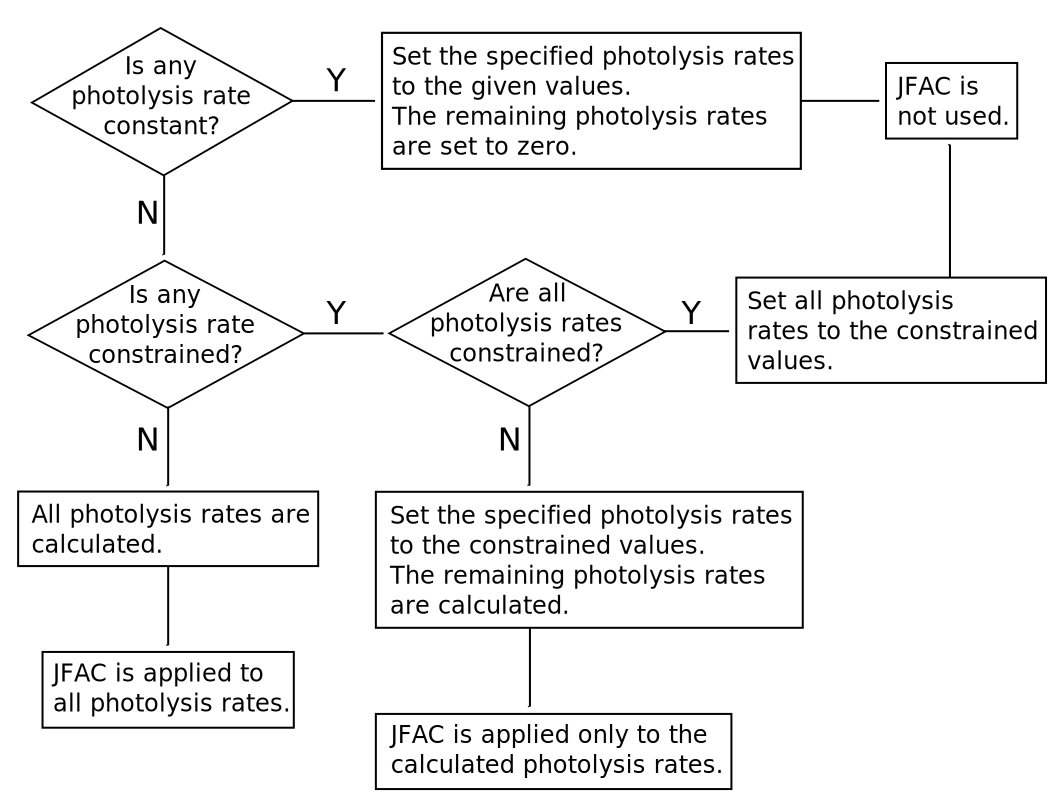
\includegraphics[width=0.5\textwidth]{photolysis.png}
  \caption{} \label{fig:}
\end{figure}

The environment variable \texttt{ROOF} can also be used to turn the
photolysis rates ON/OFF, which is useful for simulations of some
environmental chamber experiments (see
\hyperref[sec:environment-variables]{Environment Variables}).

\subsection{Constant photolysis rates} \label{subsec:constant-photolysis-rates}

The typical scenario for constant photolysis rates is the use of a
lamp in an environmental chamber. All the photolysis rates used in the
mechanism need to be given a value (in
\texttt{model/configuration/photolysisConstant.config}) otherwise they
will be set to zero. This approach allows the user to model individual
photolysis processes and/or to account for lamps that emit only in
certain spectral windows. The format of the
\texttt{photolysisConstant.config} file is described in the
\hyperref[sec:config-files]{Config Files} section.

\subsection{Constrained photolysis rates} \label{subsec:constrained-photolysis-rates}

Photolysis rates can be constrained to measured values. In this case,
the name of the constrained photolysis rate (e.g., \texttt{J2}) must
be listed in\\
\texttt{model/configuration/photolysisConstrained.config} and a
corresponding file with the constraint data must be present in
\texttt{model/constraints/photolysis/}. For more information go to:
\hyperref[sec:config-files]{Config Files} and
\hyperref[sec:constraints]{Constraints}.

It is not always possible to measure -- and therefore constrain -- all
the required photolysis rates. The photolysis rates that are not
constrained (i.e., not listed in
\texttt{photolysisConstrained.config}) are calculated using the MCM
parametrization.

\subsection{Calculated photolysis rates} \label{subsec:calculated-photolysis-rates}

AtChem2 implements the parametrization of photolysis rates used by the
Master Chemical Mechanism. It is described in the MCM protocol papers:
\citet{jenkin_1997} and \citet{saunders_2003}.

The MCM parametrization calculates the photolysis rate of a reaction
(\texttt{J}) with the equation:

\begin{verbatim}
J = l * (cosX)^m * exp(-n * secX) * tau
\end{verbatim}

where \texttt{l}, \texttt{m}, \texttt{n} are empirical parameters,
\texttt{cosX} is the cosine of the solar zenith angle, \texttt{secX}
is the inverse of \texttt{cosX} (i.e., \texttt{secX\ =\ 1/cosX}) and
\texttt{tau} is the transmission factor. The empirical parameters are
different for each version of the MCM. AtChem2 v1.1 includes the
empirical parameters for
\href{http://mcm.leeds.ac.uk/MCM/parameters/photolysis_param.htt}{version
  3.3.1} in the file \texttt{mcm/photolysis-rates\_v3.3.1}. This file
also contains the transmission factor \texttt{tau}, which can be
changed by the user (by default \texttt{tau\ =\ 1}). It is possible to
use previous versions of the MCM parametrization: see the file
\texttt{mcm/INFO.md} for instructions.

The solar zenith angle is calculated by AtChem2 using latitude,
longitude, time of the day and sun declination (see
\hyperref[sec:model-parameters]{Model Parameters} and
\hyperref[sec:environment-variables]{Environment Variables}). The
calculation is detailed in ``The Atmosphere and UV-B Radiation at
Ground Level'' \citep{madronich_1993}.

\subsection{JFAC calculation} \label{subsec:jfac-calculation}

Measurements of ambient photolysis rates typically show short-term
variability, due to the changing meteorological conditions (clouds,
rain, etc\ldots). This information is retained in the constrained
photolysis rates, but it is lost in the calculated ones. To account
for this, the calculated photolysis rates can be scaled by a
correction factor (\texttt{JFAC}), as explained below.

The environment variable \texttt{JFAC} is a constant or time-dependent
parameter that can be used to correct the calculated photolysis rates
for external factors not taken into account by the MCM
parametrization, such as cloudiness. \texttt{JFAC} is defined as the
ratio between a measured and the calculated photolysis rate. Typically
\texttt{J4} (the photolysis rate of NO2) is used for this purpose, as
it is one of the most frequently measured photolysis rates.

\begin{verbatim}
JFAC = j(NO2)/J4
\end{verbatim}

where \texttt{j(NO2)} is the measured value and \texttt{J4} is
calculated with the MCM parametrization (see above). \texttt{JFAC} is
by default 1, meaning that the calculated photolyis rates are not
scaled; it can be set to any value between 0 and 1 (see
\hyperref[sec:environment-variables]{Environment Variables}) or it can
be constrained (see \hyperref[sec:constraints]{Constraints}). Note
that only the photolysis rates calculated with the MCM parametrization
are scaled by \texttt{JFAC}, the constrained and the constant
photolysis rates are not.

\texttt{JFAC} can also be calculated at runtime. To do so,
\texttt{JFAC} should be set to the name of the photolysis rate to be
used as reference (e.g., \texttt{J4}) in\\
\texttt{model/configuration/environmentVariables.config}. There should
be an associated constraint file in
\texttt{model/constraints/environment/}. \textbf{Important}: this
option is not working very well in the current version of AtChem2, so
it is suggested to calculate \texttt{JFAC} offline and to constrain it
(see issue \href{https://github.com/AtChem/AtChem2/issues/16}{\#16}).

% -------------------------------------------------------------------- %
\section{Config Files} \label{sec:config-files}

The \textbf{configuration files} contain the settings for the initial
conditions, the constraints and the output of the model. These files
complement the configuration settings of the model (in
\texttt{model.parameters}) and of the solver (in
\texttt{solver.parameters}), which are in the same directory. For more
information go to: \hyperref[sec:model-parameters]{Model Parameters} and
\hyperref[sec:solver-parameters]{Solver Parameters}).

The configuration files have the extension \texttt{.config} and, by
default, are in the directory \texttt{model/configuration/}. This
directory also contains the files generated during the
\hyperref[subsec:build-process]{build process} which describe the
chemical mechanism (\texttt{mechanism.species},
\texttt{mechanism.reac}, \texttt{mechanism.prod},
\texttt{mechanism.ro2}), as explained in the
\hyperref[sec:chemical-mechanism]{Chemical Mechanism} page. The location of the
configuration files can be modified by changing the arguments of the
script \texttt{build/build\_atchem2.sh} (see
\hyperref[subsec:build-process]{Build Process}).

The content and the format of the \texttt{.config} files are described
below. Note that the names of some files have changed with the release
of \textbf{version 1.1} (November 2018).

\subsection{environmentVariables.config} \label{subsec:environmentvariables}

This file contains the settings for the environment variables, which
are described in detail in the related
\hyperref[sec:environment-variables]{section}. If an environment variable is
constrained, there must be a corresponding data file in
\texttt{model/constraints/environment/} (see
\hyperref[sec:constraints]{Constraints}).

\subsection{initialConcentrations.config} \label{subsec:initialconcentrations}

This file contains the initial concentrations of the chemical species.
The first column is the list of initialized species, the second column
is the corresponding concentration at \texttt{t\ =\ 0} (in
\textbf{molecules cm-3}). For example:

\begin{verbatim}
NO      378473308.14
NO2     86893908168.9
O3      1.213e+12
CH4     4.938e+13
\end{verbatim}

The chemical species not included in this file are automatically
initialized to the default value \texttt{0}. It is not necessary to
initialize the constant and the constrained species (i.e., those
listed in \texttt{speciesConstant.config} and
\texttt{speciesConstrained.config}).

The environment variables are set in
\texttt{environmentVariables.config} (see above) and should not be
included in this file.

\subsection{outputRates.config} \label{subsec:outputrates}

This file (called \texttt{productionRatesOutput.config} and
\texttt{lossRatesOutput.config} in v1.0) lists the chemical species
for which detailed production rates and loss rates are required. The
file has one column, with one species per line.

The frequency of this output is controlled by the \textbf{rates output
  step size} parameter in \texttt{model.parameters} (see
\hyperref[sec:model-parameters]{Model Parameters}). The format of the
corresponding output files -- \texttt{lossRates.output} and
\texttt{productionRates.output} -- is designed to facilitate the
analysis of production and destruction rates for selected species of
interests (rather than processing the output files generated in
\texttt{model/output/reactionRates/}):

\newpage
\begin{scriptsize}
\begin{verbatim}
     time        speciesNumber    speciesName    reactionNumber         rate        reaction

3.600000E+003           8               OH              15         0.000000E+000    O1D=OH+OH
3.600000E+003           8               OH              20         0.000000E+000    HO2+O3=OH
3.600000E+003           9               HO2             16         0.000000E+000    OH+O3=HO2
3.600000E+003           9               HO2             17         0.000000E+000    OH+H2=HO2

7.200000E+003           8               OH              15         0.000000E+000    O1D=OH+OH
7.200000E+003           8               OH              20         0.000000E+000    HO2+O3=OH
7.200000E+003           9               HO2             16         0.000000E+000    OH+O3=HO2
7.200000E+003           9               HO2             17         0.000000E+000    OH+H2=HO2
\end{verbatim}
\end{scriptsize}

\subsection{outputSpecies.config} \label{subsec:outputspecies}

This file (called \texttt{concentrationOutput.config} in v1.0) lists
the chemical species for which the model output is required. The
current version of AtChem2 limits the number of species that can be
output to 100, although the user can modify the Fortran code to
increase this number. The file has one column, with one species per
line.

The frequency of this output is controlled by the \textbf{step size}
parameter in \texttt{model.parameters} (see
\hyperref[sec:model-parameters]{Model Parameters}).

\subsection{photolysisConstant.config} \label{subsec:photolysisconstant}

This file lists the photolysis rates that are constant. The file has
three columns: the first column is the number that identifies the
photolysis rate (e.g., \texttt{1}), the second column is the value of
the photolysis rate in \textbf{s-1} (e.g., \texttt{1e-5}), the third
column is the name of the photolysis rate (e.g., \texttt{J1}). The
photolysis rates are named according to the
\href{http://mcm.leeds.ac.uk/MCM/parameters/photolysis.htt}{MCM
  naming convention}. If no photolysis rate is constant, the file
should be left empty.

If one or more photolysis rates is set to a constant value, the others
(i.e., those not listed in \texttt{photolysisConstants.config}) are
set to zero. For more information go to:
\hyperref[sec:photolysis-rates]{Photolysis Rates and JFAC}.

\subsection{photolysisConstrained.config} \label{subsec:photolysisconstrained}

This file (called \texttt{constrainedPhotoRates.config} in v1.0) lists
the photolysis rates that are constrained. The file has one column,
with one photolysis rate per line (e.g., \texttt{J1}). The photolysis
rates are named according to the
\href{http://mcm.leeds.ac.uk/MCM/parameters/photolysis.htt}{MCM
  naming convention}. If no photolysis rate is constrained, the file
should be left empty. If a photolysis rate is constrained, there must
be a corresponding data file in \texttt{model/constraints/photolysis/}
(see \hyperref[sec:constraints]{Constraints}).

The photolysis rates that are not listed in
\texttt{photolysisConstrained.config} are calculated by AtChem2 using
the MCM parametrization and the parameters in
\texttt{mcm/photolysis-rates\_v3.3.1}. Older versions of the MCM
photolysis parametrization can be used, as explained in the file
\texttt{mcm/INFO.md}. For more information go to:
\hyperref[sec:photolysis-rates]{Photolysis Rates and JFAC}.

\subsection{speciesConstant.config} \label{subsec:speciesconstant}

This file (called \texttt{constrainedFixedSpecies.config} in v1.0)
lists the chemical species that are constant. The file has two
columns: the first column is the list of constant species, the second
column is the corresponding concentration (in \textbf{molecules
  cm-3}). If no chemical species is constant, the file should be left
empty.

If a chemical species is constant, it does not need to be initialized:
the values set in \texttt{speciesConstant.config} override those set
in \texttt{initialConcentrations.config}.

\subsection{speciesConstrained.config} \label{subsec:speciesconstrained}

This file (called \texttt{constrainedSpecies.config} in v1.0) lists
the chemical species that are constrained. The file has one column,
with one species per line. If no chemical species is constrained, the
file should be left empty. If a chemical species is constrained, there
must be a corresponding data file in
\texttt{model/constraints/species/} (see
\hyperref[sec:constraints]{Constraints}).

If a chemical species constrained, it does not need to be initialized:
the values set in \texttt{speciesConstrained.config} override those
set in \texttt{initialConcentrations.config}.

% -------------------------------------------------------------------- %
\section{Constraints} \label{sec:constraints}

AtChem2 can be run in two modes:

\begin{itemize}
\item unconstrained: all variables are calculated by the model from
  the initial conditions, set in the \hyperref[sec:config-files]{model
    configuration files}.
\item constrained: one or more variables are constrained, i.e. the
  solver forces their value to a given value. The variables that are
  not constrained are calculated by the model.
\end{itemize}

The constrained values must be provided as separate files for each
constrained variable. The format of the constraint files is described
below. By default, the files with the constraining data are in
\texttt{model/constraints/species/} for the chemical species,
\texttt{model/constraints/environment/} for the environment variables,
and \texttt{model/constraints/photolysis/} for the photolysis
rates. The default directories can be modified by changing the
arguments of the \texttt{atchem2} executable (see
\hyperref[sec:execute]{Execute}).

\subsection{Constrained variables} \label{subsec:constrained-variables}

\subsubsection{Environment variables}

All environment variables, except \texttt{ROOF}, can be
constrained. To do so, set the variable to \texttt{CONSTRAINED} in
\texttt{model/configuration/environmentVariables.config} and create
the file with the constraining data. The name of the file must be the
same as the name of the variable, e.g., \texttt{TEMP} (without
extension). See also: \hyperref[sec:environment-variables]{Environment Variables}.

\subsubsection{Chemical species}

Any chemical species in the chemical mechanism can be constrained. To
do so, add the name of the species to
\texttt{model/configuration/speciesConstrained.config} and create the
file with the constraining data. The name of the file must be the same
as the name of the chemical species, e.g., \texttt{CH3OH} (without
extension). See also: \hyperref[sec:config-files]{Config Files}.

\subsubsection{Photolysis rates}

Any of the photolysis rates in the chemical mechanism can be
constrained. The photolysis rates are identified as \verb|J<n>|, where
\texttt{n} is an integer (see
\hyperref[sec:photolysis-rates]{Photolysis Rates and JFAC}). To
constrain a photolysis rate add its name (\texttt{Jn}) to\\
\texttt{model/configuration/photolysisConstrained.config} and create
the file with the constraining data. The name of the file must be the
same as the name of the photolysis rate, e.g., \texttt{J4} (without
extension). See also \hyperref[sec:config-files]{Config Files}.

\subsection{Constraint files} \label{subsec:constraint-files}

The files with the constraining data are text files with two columns
separated by spaces. The first column is the time in \textbf{seconds}
from midnight of day/month/year (see \hyperref[sec:model-parameters]{Model
  Parameters}), the second column is the value of the variable in the
appropriate unit. For the chemical species the unit is
\textbf{molecules cm-3} and for the photolysis rates the unit is
\textbf{s-1}; for the environment variables see the related
\hyperref[sec:environment-variables]{section}. For example:

\begin{verbatim}
-900   73.21
0      74.393
900    72.973
1800   72.63
2700   72.73
3600   69.326
4500   65.822
5400   63.83
6300   64.852
7200   64.739
\end{verbatim}

The time in the first column of a constraint file can be negative.
AtChem2 interprets the negative timestamps as ``seconds \emph{before}
midnight of day/month/year'' (see \hyperref[sec:model-parameters]{Model
  Parameters}). This can be useful to allow correct interpolation of
the variables at the beginning of the model run (see below).

\textbf{Important.} The constraints must cover the same amount of
time, or preferably more, as the intended model runtime. For example:
if the model starts at 42300 seconds and stops at 216000 seconds, the
first and the last data points in a constraint file must have a
timestamp of 42300 (or lower) and 21600 (or higher), respectively.

\subsection{Interpolation} \label{subsec:interpolation}

Constraints can be provided at different timescales. Typically, the
constraining data come from direct measurements and it is a very
common for different instruments to sample at different
frequencies. For example, ozone and nitrogen oxides can be measured
once every minute, but most organic compounds can be measured only
once every hour.

The user can average the constraints so that they are all at the same
timescale or can use the data with the original timestamps. Both
approaches have advantages and disadvantages in terms of how much
pre-processing work is required, and in terms of model accuracy and
integration speed. Whether all the constraints have the same timescale
or not, the solver interpolates between data points using the
interpolation method selected in the
\texttt{model/configuration/model.parameters} file (see
\hyperref[sec:model-parameters]{Model Parameters}). The default
interpolation method is piecewise linear, but piecewise constant
interpolation is also available.

The photolysis rates and the environment variables are evaluated by
the solver when needed -- each is interpolated individually, only when
constrained. This happens each time the function
\texttt{mechanism\_rates()} is called from \texttt{FCVFUN()}, and
therefore is controlled by \textbf{CVODE} as it completes the
integration. In a similar way, the interpolation routine for the
chemical species is called once for each of the constrained species in
\texttt{FCVFUN()}, plus once when setting the initial conditions of
each of the constrained species.

As mentioned above, the model start and stop time \emph{must be}
within the time interval of the constrained data to avoid
interpolation errors or model crash. If data is not supplied for the
full runtime interval, then the \emph{final} value will be used for
all times both \emph{before the first data point} and \emph{after the
  last data point}. This behaviour is likely to change in future
versions, at least to avoid the situation where the last value is used
for all times before the first (see issue
\href{https://github.com/AtChem/AtChem2/issues/294}{\#294}).

A warning is printed for all evaluations outside of the supplied time
interval. Users may find it useful to supply data that covers a short
time \emph{beyond} the final model time, which may be used by the
solver.
